\documentclass{article}

\usepackage{graphicx}
\usepackage{tikz}
\usepackage{tikzsymbols}
\usetikzlibrary{calc,patterns,shapes.geometric}
\pagestyle{empty}
\usepackage[margin=0pt]{geometry}
\geometry{papersize={14in,12in}}

\def\centerarc[#1](#2)(#3:#4:#5){\draw[#1] ($(#2)+({#5*cos(#3)},{#5*sin(#3)})$) arc (#3:#4:#5);}

\begin{document}
	\begin{figure}
		\centering
		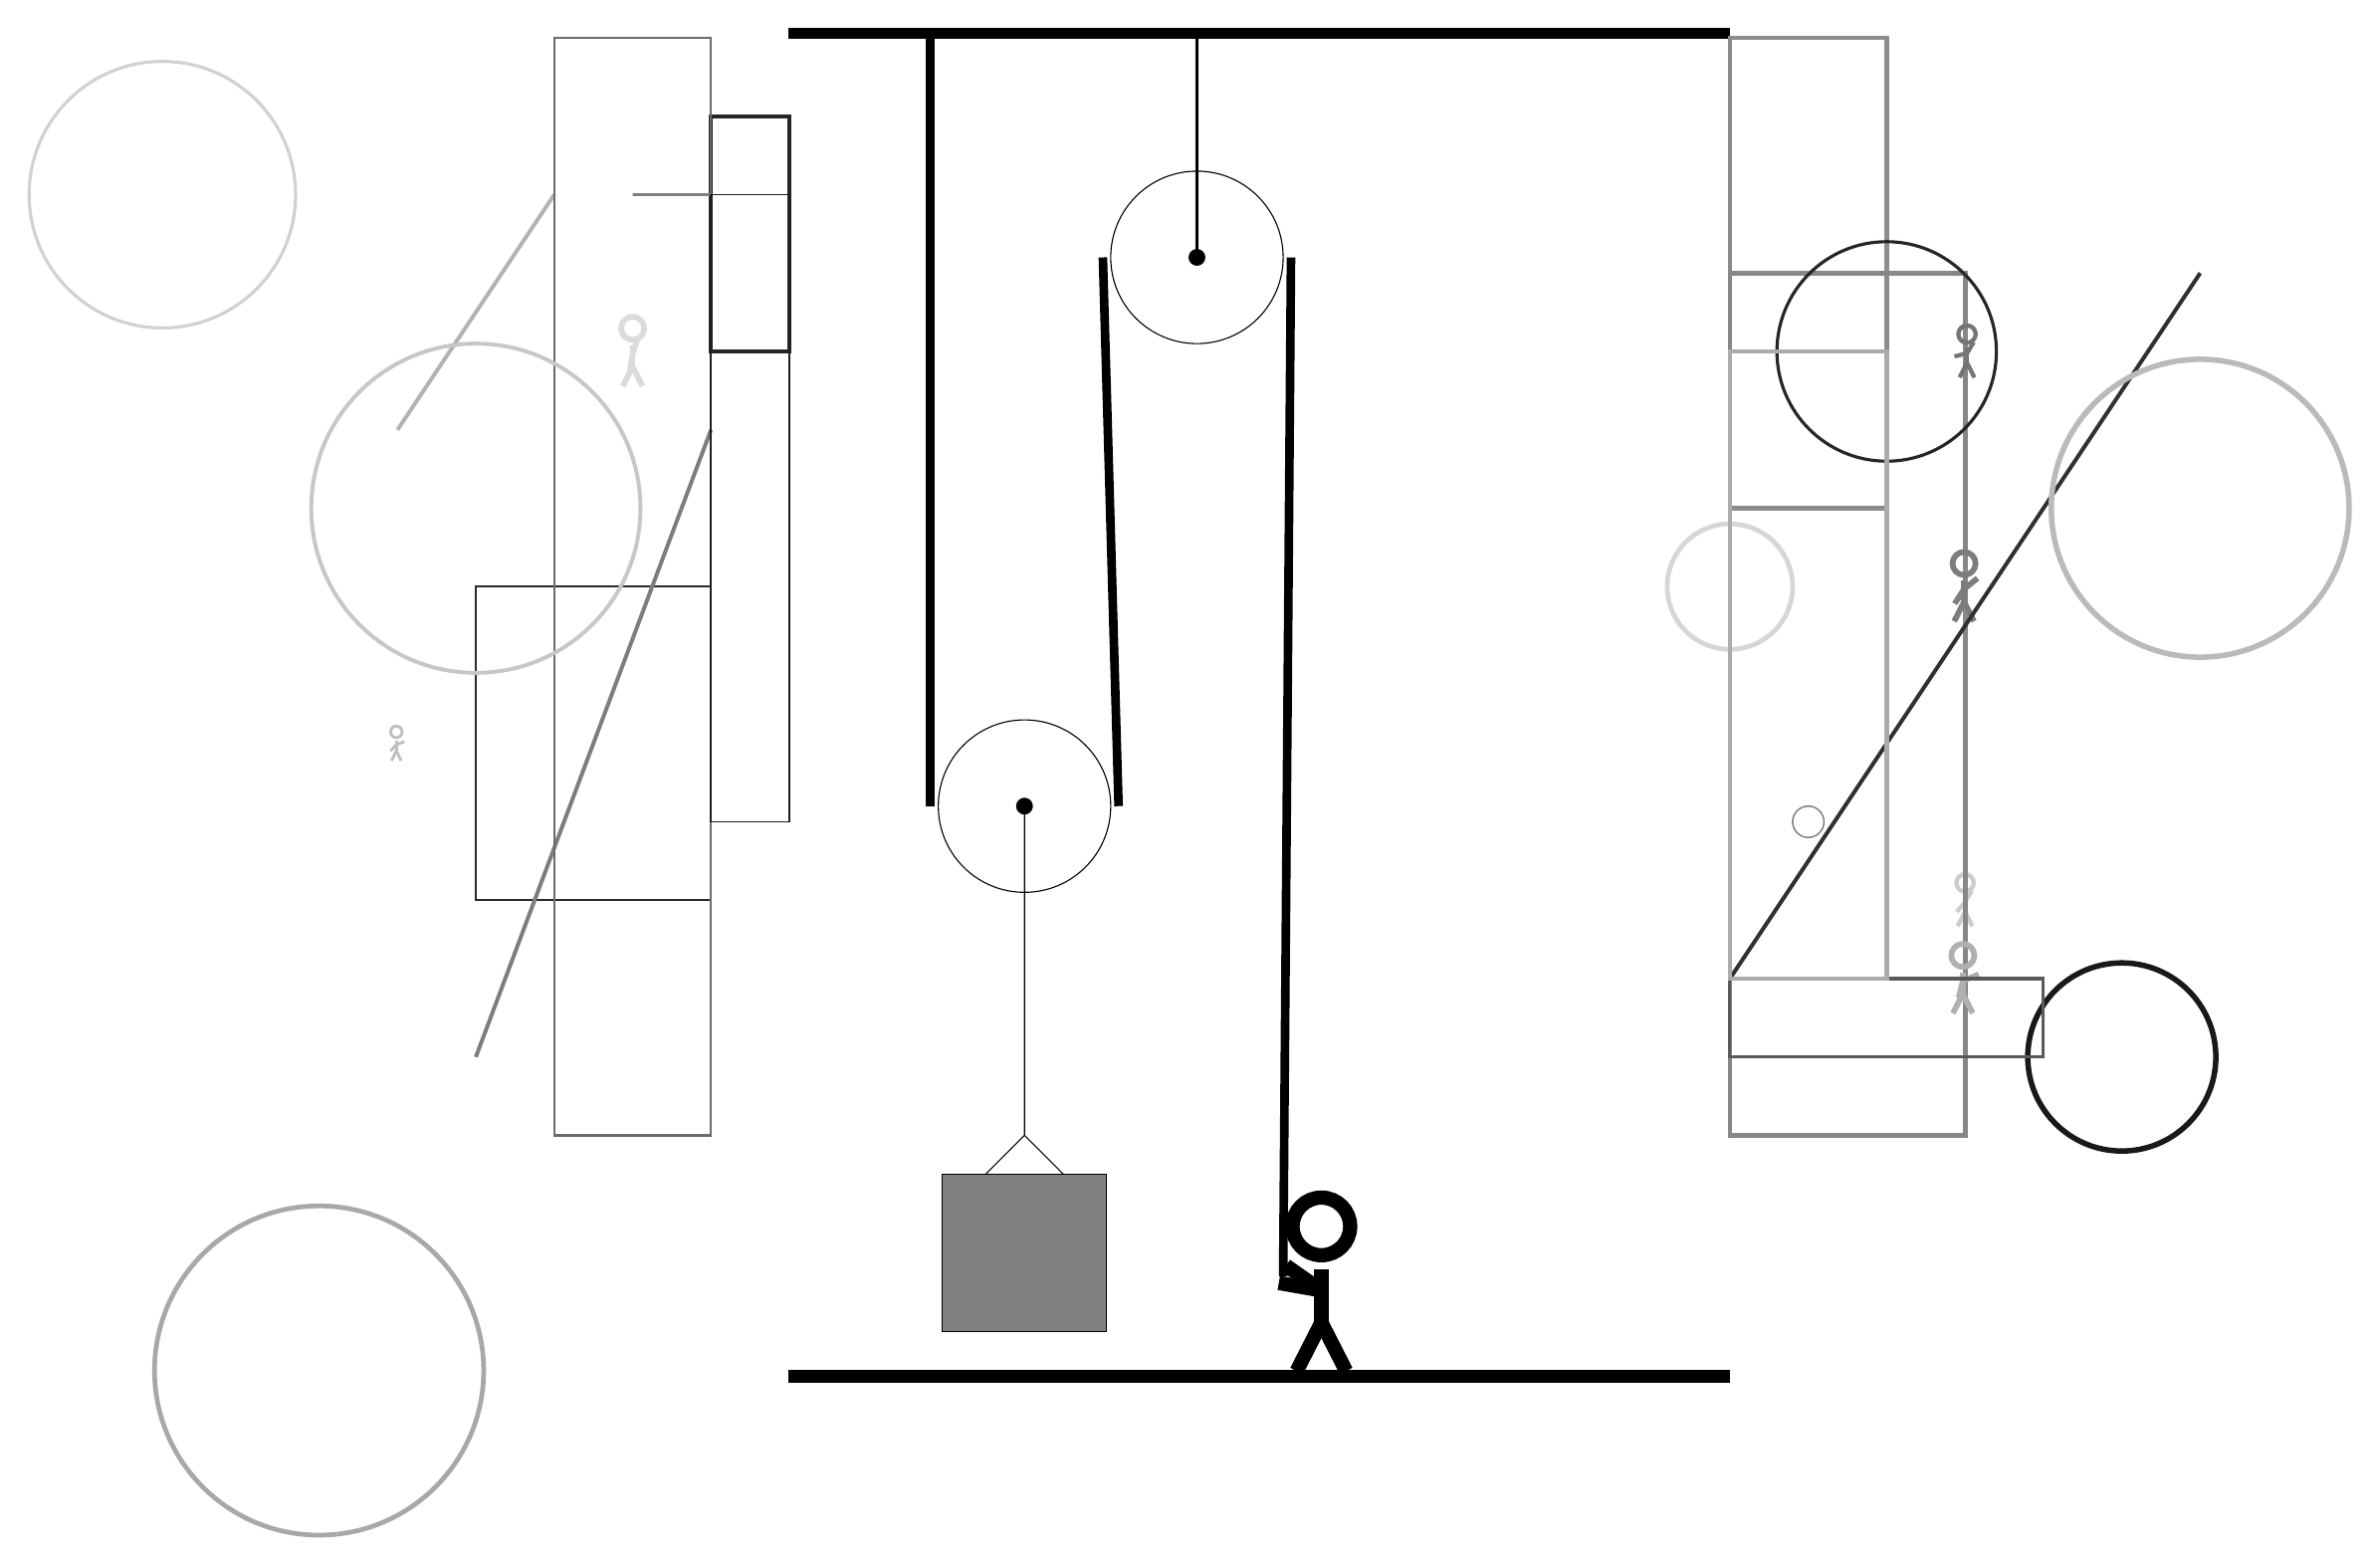
\begin{tikzpicture}
			%%%%% START %%%%%
			
			\draw[fill=black] (-2, 14) rectangle (10, 14.125);
			
			\draw (3.2, 11.2) circle (1.1);
			\draw[fill=black] (3.2, 11.2) circle (0.1);
			\draw[thick] (3.2, 11.2) -- (3.2, 14);
			
			\draw (1, 4.2) circle (1.1);
			\draw[fill=black] (1, 4.2) circle (0.1);
			
			\draw (1, 4.2) -- (1, 0) -- (0.5, -0.5);
			\draw (1, 0) -- (1.5, -0.5);
			\draw[fill=black!50] (-0.05, -0.5) rectangle (2.05, -2.5);
			
			\draw [line width=0.6mm, color=black!20](11, 6) circle (0.0);
			
			\draw [line width=0.7mm, color=black!90](15, 1) circle (1.2);
			\draw [line width=0.6mm, color=black!16](10, 7) circle (0.8);
			\draw[line width=0.2mm, color=black!85] (-3, 6) rectangle (-3, 14);
			
			\draw[line width=0.2mm, color=black!84] (-3, 3) rectangle (-6, 7);
			\draw[line width=0.6mm, color=black!45] (12, 8) rectangle (10, 14);
			
			\node[line width=0.6mm, color=black!20] at (13, 3) {\Strichmaxerl[3][50][59]};
			\draw[line width=0.6mm, color=black!47] (10, 11) rectangle (13, 0);
			\draw[line width=0.5mm, color=black!85] (-3, 10) rectangle (-2, 13);
			
			\draw[line width=0.3mm, color=black!86] (-2, 7) rectangle (-2, 9);
			
			\draw[line width=0.5mm, color=black!30](-7, 9) -- (-5, 12);
			
			\draw[line width=0.5mm, color=black!51](-3, 9) -- (-6, 1);
			\draw[line width=0.3mm, color=black!58] (-3, 14) rectangle (-5, 0);
			
			\node[line width=0.2mm, color=black!51] at (13, 7) {\Strichmaxerl[4][57][39]};
			\draw [line width=0.4mm, color=black!85](12, 10) circle (1.4);
			\draw [line width=0.4mm, color=black!18](-10, 12) circle (1.7);
			
			\draw[line width=0.4mm, color=black!50] (-3, 12) rectangle (-4, 12);
			\draw[line width=0.5mm, color=black!81](10, 2) -- (16, 11);
			\draw [line width=0.2mm, color=black!48](11, 4) circle (0.2);
			\node[line width=0.6mm, color=black!31] at (13, 2) {\Strichmaxerl[4][76][23]};
			\draw[line width=0.4mm, color=black!65] (10, 2) rectangle (14, 1);
			
			\node[line width=0.2mm, color=black!14] at (-4, 10) {\Strichmaxerl[4][81][72]};
			\draw[line width=0.2mm, color=black!88] (-2, 12) rectangle (-3, 4);
			\draw [line width=0.7mm, color=black!27](16, 8) circle (1.9);
			\node[line width=0.7mm, color=black!25] at (-7, 5) {\Strichmaxerl[2][48][20]};
			
			\draw [line width=0.5mm, color=black!22](-6, 8) circle (2.1);
			
			\draw[line width=0.6mm, color=black!33] (12, 10) rectangle (10, 2);
			\draw [line width=0.6mm, color=black!34](-8, -3) circle (2.1);
			\node[line width=0.2mm, color=black!54] at (13, 10) {\Strichmaxerl[3][14][59]};
			
			\draw[line width=1.1mm] (-0.2, 14) -- (-0.2, 4.2);
			\centerarc[line width=1.1mm](1, 4.2)(180:360:1.2000000000000002);
			\draw[line width=1.1mm](2.2, 4.2) -- (2.0, 11.2);
			\centerarc[line width=1.1mm](3.2, 11.2)(0:180:1.2000000000000002);
			\draw[line width=1.1mm](4.4, 11.2) -- (4.3, -1.8);
			
			\node at (4.7, -1.9) {\Strichmaxerl[10][-35][170]};
			
			\draw[fill=black] (-2, -3) rectangle (10, -3.15);
			
			%%%%% END %%%%%
		\end{tikzpicture}
	\end{figure}	
\end{document}